\section{Theoretical predictions for the neutral pion polarizability}
The low energy properties of pions are largely determined by  their nature as
the Goldstone Bosons of spontaneously broken chiral symmetry in QCD,
and are described in a model independent way by the framework of
Chiral Perturbation Theory (ChPT) (Gasser and Leutwyler
\cite{Gasser:1983yg}), which implements a systematic expansion in low
energy/momentum and in quark masses.  In particular the pions' low
energy electromagnetic properties can serve as tests of their
Goldstone Boson (GB) nature. One such a case is the $\pi^0\to
\gamma\gamma$ decay, which at the same time tests its GB nature and
the chiral anomaly. Another case is low energy Compton scattering on
pions: at low energy the Compton differential cross section can be
expanded in powers of the photon energy and expressed in terms of the
corresponding pion charge form factor (for charged pion) and the electric
and magnetic
polarizabilities, where the latter give the order $\omega^2$ terms in
the Compton cross section, being $\omega$ the photon energy. The
polarizabilities appear as deviations
of the pions from point like particles, and thus result from carrying
out the chiral expansion to the next-to-leading order. For both
charged an neutral pions the polarizabilities are fully predicted at
leading order in quark masses, and thus represent a sensitive test of
chiral dynamics. For the charged pions, at $O(p^4)$ ChPT predicts that
the electric and magnetic polarizabilities ($\alpha_{\pi^+}$ and
$\beta_{\pi^+}$) are related to the charged pion weak form factors
$F_V$ and $F_A$ in the decay $\pi^+ \rightarrow e^+ \nu \gamma$
\begin{equation}\label{alpha_and_beta}
\alpha_{\pi^+} = -\beta_{\pi^+} \propto \frac{F_A}{F_V} = \frac{1}{6} ( l_6 - l_5 ),
\end{equation}

\noindent where $l_5$ and $l_6$ are low energy constants in the Gasser
and Leutwyler effective Lagrangian \cite{Gasser:1983yg}.  Using recent
results from the PIBETA collaboration for $F_A$ and $F_V$
\cite{Bychkov:2008ws}, the $O(p^4)$ ChPT prediction for the charged
pion electric and magnetic polarizabilities is given by:
\begin{equation}\label{one_loop}
\alpha_{\pi^+} = -\beta_{\pi^+} = (2.78 \pm 0.1) \times 10^{-4}~{\rm fm}^3.
\end{equation}

\begin{figure}[h]
\begin{center}
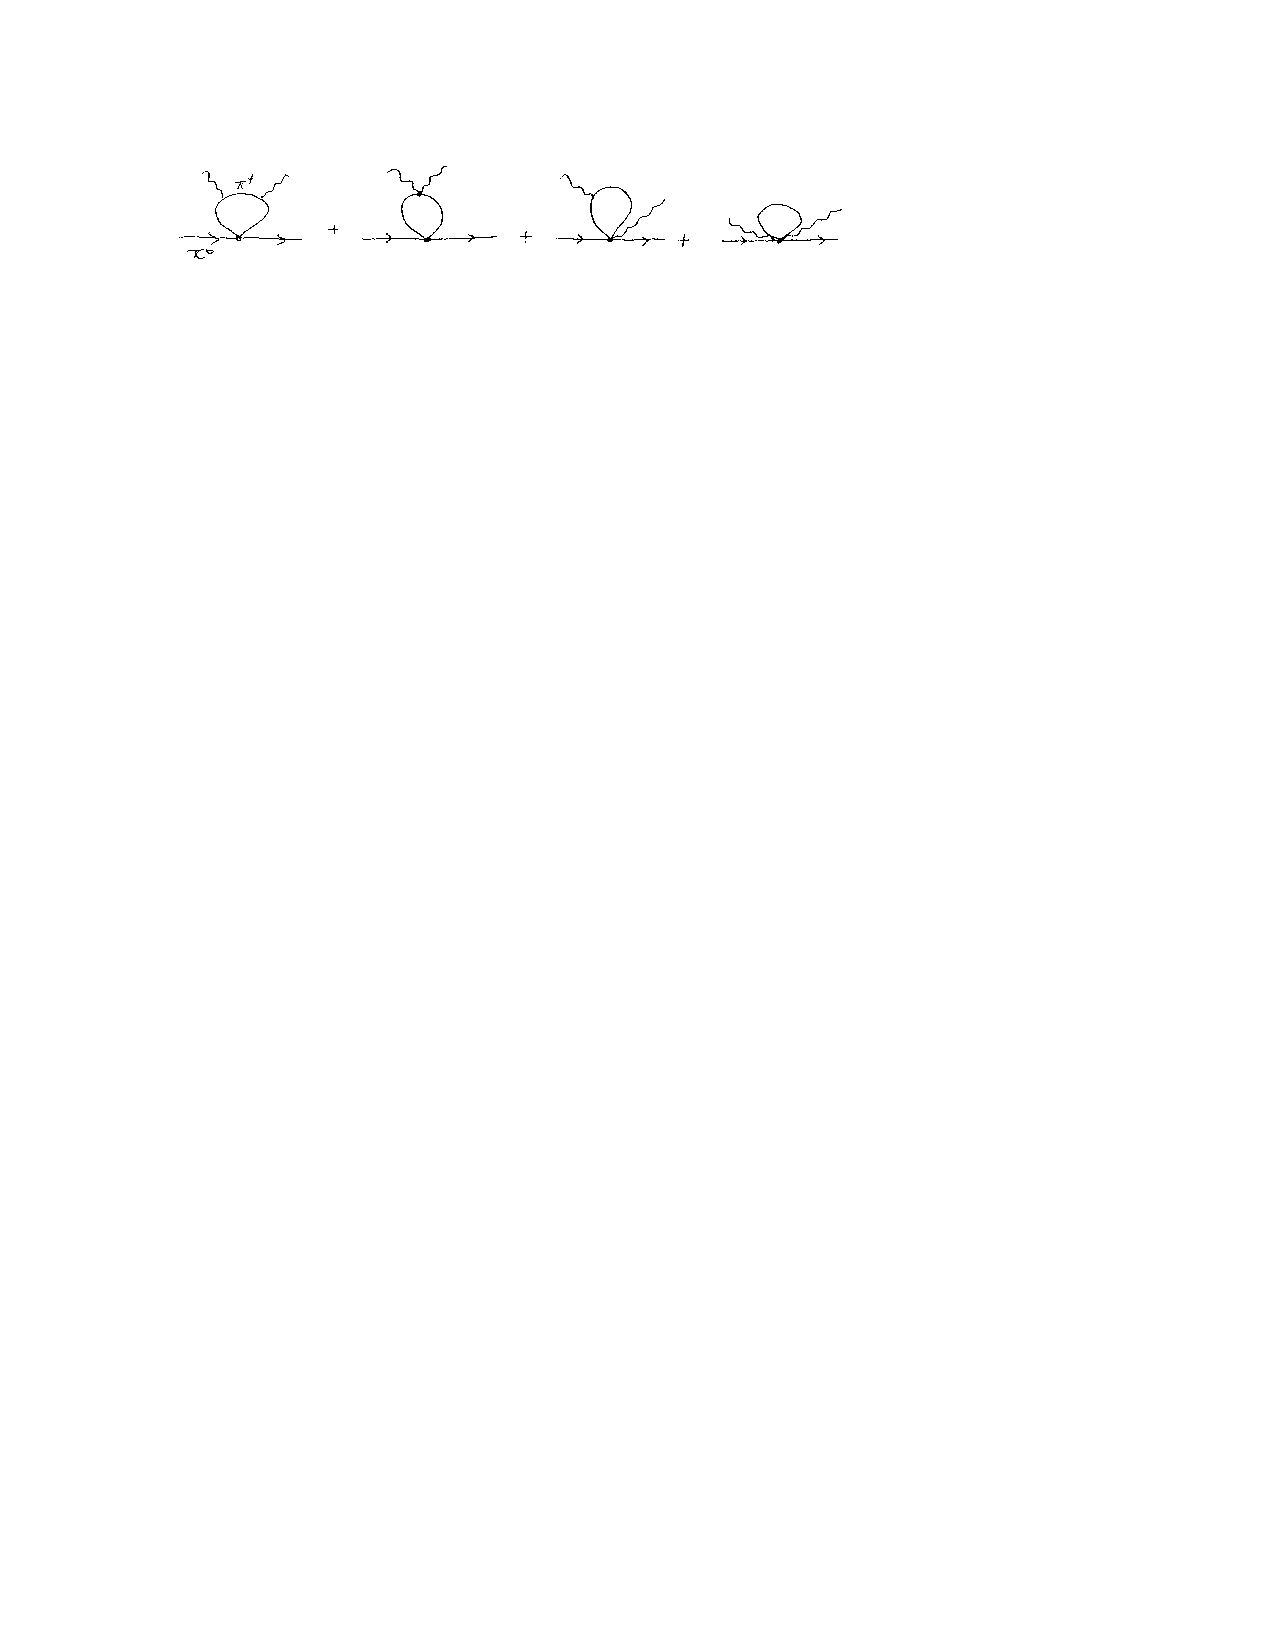
\includegraphics[height=2cm,angle=0]{figures/Fig-TP-1.pdf}
%\includegraphics[height=6cm,width=8cm,angle=0]{gA-Mpi-LHPC-band.pdf}
\end{center}
\caption{Diagrams contributing to Compton scattering off the $\pi^0$.
\label{fig:digrams}}
\end{figure}


In the case of the neutral pion, the polarizabilities are determined
by the one loop chiral contributions (see Fig.\,\ref{fig:digrams})
which are calculable, free of unknown parameters, and given only in
terms of the fine structure constant, the pion mass and the pion decay
constant:
\begin{eqnarray}
\alpha_{\pi^0}+\beta_{\pi^0}&=&0\nonumber\\
\alpha_{\pi^0}-\beta_{\pi^0}&=&-\frac{\alpha}{48 \pi^2 M_\pi F_\pi^2}\simeq -1.1\times 10^{-4}~{\rm fm}^3
\end{eqnarray}
However, there is a range of predictions beyond
NLO and the experimental test of these important predictions is very
challenging. In the first place, the polarizabilities drive the very
low energy regime of Compton scattering on the $\pi^0$ as there is no
Thomson term, so one would expect that it would be easier to determine
them than in the charged pion case.  However, in the first place
Compton scattering on the $\pi^0$ is experimentally inaccessible due
to its short lifetime, and therefore it is necessary to resort to the
process $\gamma\gamma\to \pi^0\pi^0$ of this proposal. In addition, ChPT
indicates that the
polarizabilities are smaller in the case of the neutral pion, about a
third of their value for the charged pion, i.e. somewhere between
$-1.7\times 10^{-4}~{\rm fm}^3$ and $-1.9\times 10^{-4}~{\rm fm}^3$,
depending on the model used to estimate higher order effects in the chiral
expansion. The challenge is therefore to measure the
cross section for $\gamma\gamma \to \pi^0\pi^0$ with sufficient
accuracy at low invariant mass $W_{\pi\pi}$ so that one can infer the
low-energy Compton amplitude and extract the polarizabilities. The demand for
accuracy is required in order to allow for the extrapolation of the Compton
amplitude from the kinematics of $\gamma\gamma \to \pi^0\pi^0$ to   low energy
Compton scattering, something that is at present impossible with the poor
accuracy of the only available data from the Crystal Ball experiment \cite{}.
 


For
this purpose, the theoretical foundations have been laid in works
studying $\gamma\gamma\to \pi^0\pi^0$ both using ChPT (Bellucci et al
\cite{Bellucci:1994hx,Bellucci:1994eb}, Gasser et al
\cite{Gasser:2005ud}, Aleksejevs and Barkanova
\cite{Aleksejevs:2014eea}) and dispersion theory (Oller and Roca
\cite{Oller:2008kf}, Dai and Pennington
\cite{Dai:2014zta,Dai:2014lza}, Moussallam
\cite{Moussallam:2013una}). In particular, in ChPT at the next-to-next
to leading order, which provides the higher order quark mass
corrections to the polarizabilities, some of the low energy constants
need to be fixed and for that a significantly more accurate
measurement of the $\gamma\gamma\to \pi^0\pi^0$ cross section is
needed than available presently.

Accurate measurements of the cross section near threshold combined
with data for $W_{\pi\pi}>0.6$ GeV will provide the necessary input
for performing a full theoretical analysis, combining dispersion
theory with and without inputs from ChPT at low energy. This is a well
established method which has been used to analyze $\pi\pi$
scattering and also to the very problem of the $\gamma\gamma \to \pi^0\pi^0$
process, where numerous works have been steadily improved the theoretical
dispersive analysis, to mention a
few \cite{Donoghue:1993kw,Oller:2007sh,Oller:2008k,Moussallam:2013una,Dai:2016ytz}.
Through such an analysis it will be possible to determine,
via combination with ChPT, the low energy Compton amplitude and
extract the   combination $\alpha_\pi-\beta_\pi$. The
latter extraction represents a challenge as shown in
Fig.\,\ref{fig:previousdata}, where the polarizabilities have a small
direct effect on $\gamma\gamma\to \pi\pi$.  Calculations by Dai and
Pennington (Table II) \cite{Dai:2016ytz} indicate that a 1.3\%
determination of $\sigma(\gamma\gamma\rightarrow\pi^0\pi^0)$ will
determine the combination of $\alpha_{\pi^0}-\beta_{\pi^0}$ to a
precision of 10\%. 
%The preliminary study done by Aleksejevs and Barkanova for this proposal in relativistic ChPT with SU(3) input indicate that sensitivity could be even better depending on specific kinematics; the full evaluation is in progress. 
In general, the
determination of the accuracy one can get for $\alpha_\pi-\beta_\pi$
based on a more accurate measurement as the one proposed here is still
an issue being currently studied theoretically, with J. L.  Goity and
A. Aleksejevs and S. Barkanova forming a group to take a lead on the project. 
At present a theoretical study based on the S-wave dominance below
$W_{\pi\pi}\sim 0.8 GeV$ and dispersion theory has allowed to represent the two
Compton amplitudes $A$ and $B$ in the physical domain of the experiment. The
study of the extrapolation to low energy Compton kinematics is under study, in
particular the issues related to the stability of the dispersive analysis. This
study is expected to provide a more accurate estimate on the sensitivity with
which the experiment will allow for the determination of the polarizability
$\alpha-\beta$.


%However, even 10\% precision would still be sufficient to difference between various models and facilitate extraction of low-energy constants, and thus a highly desirable result for theory.

\begin{figure}[ht]
\begin{center}
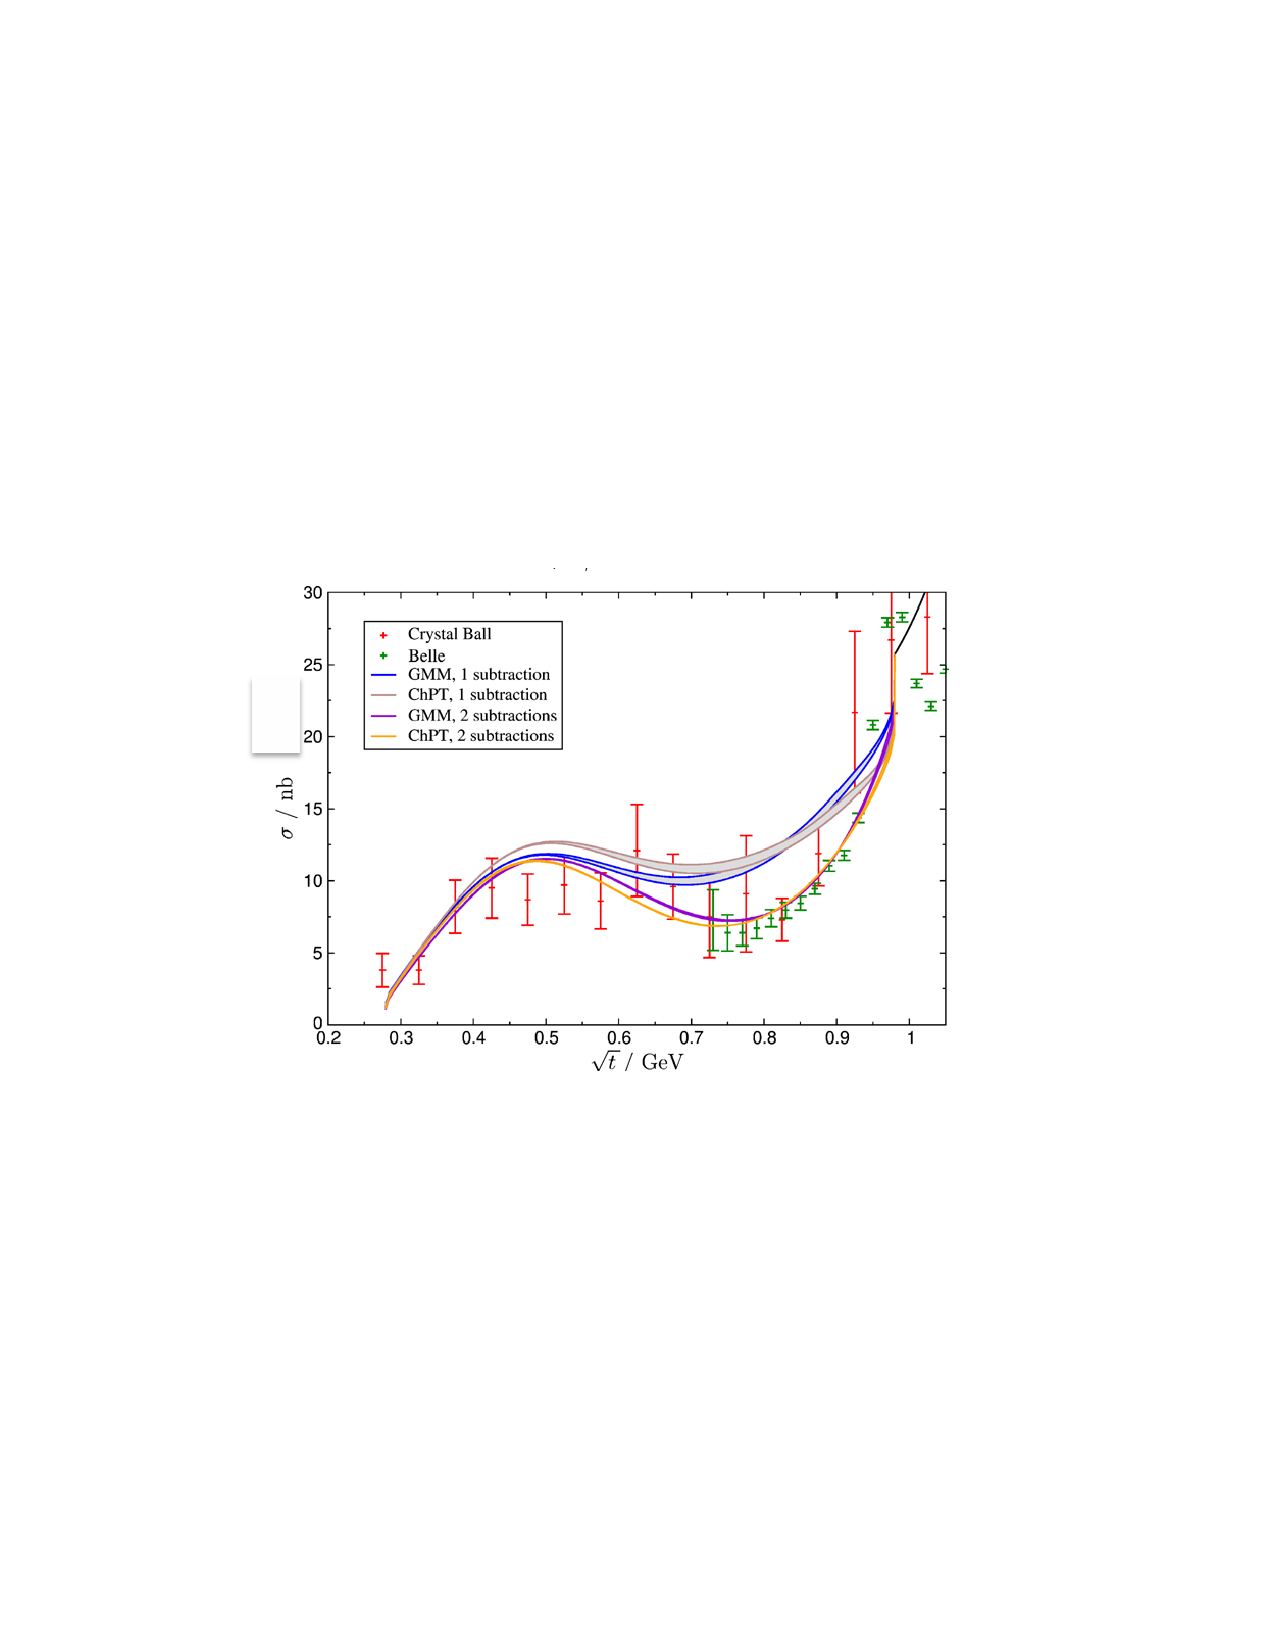
\includegraphics[height=5cm,angle=0]{figures/Fig-TP-2pr.pdf}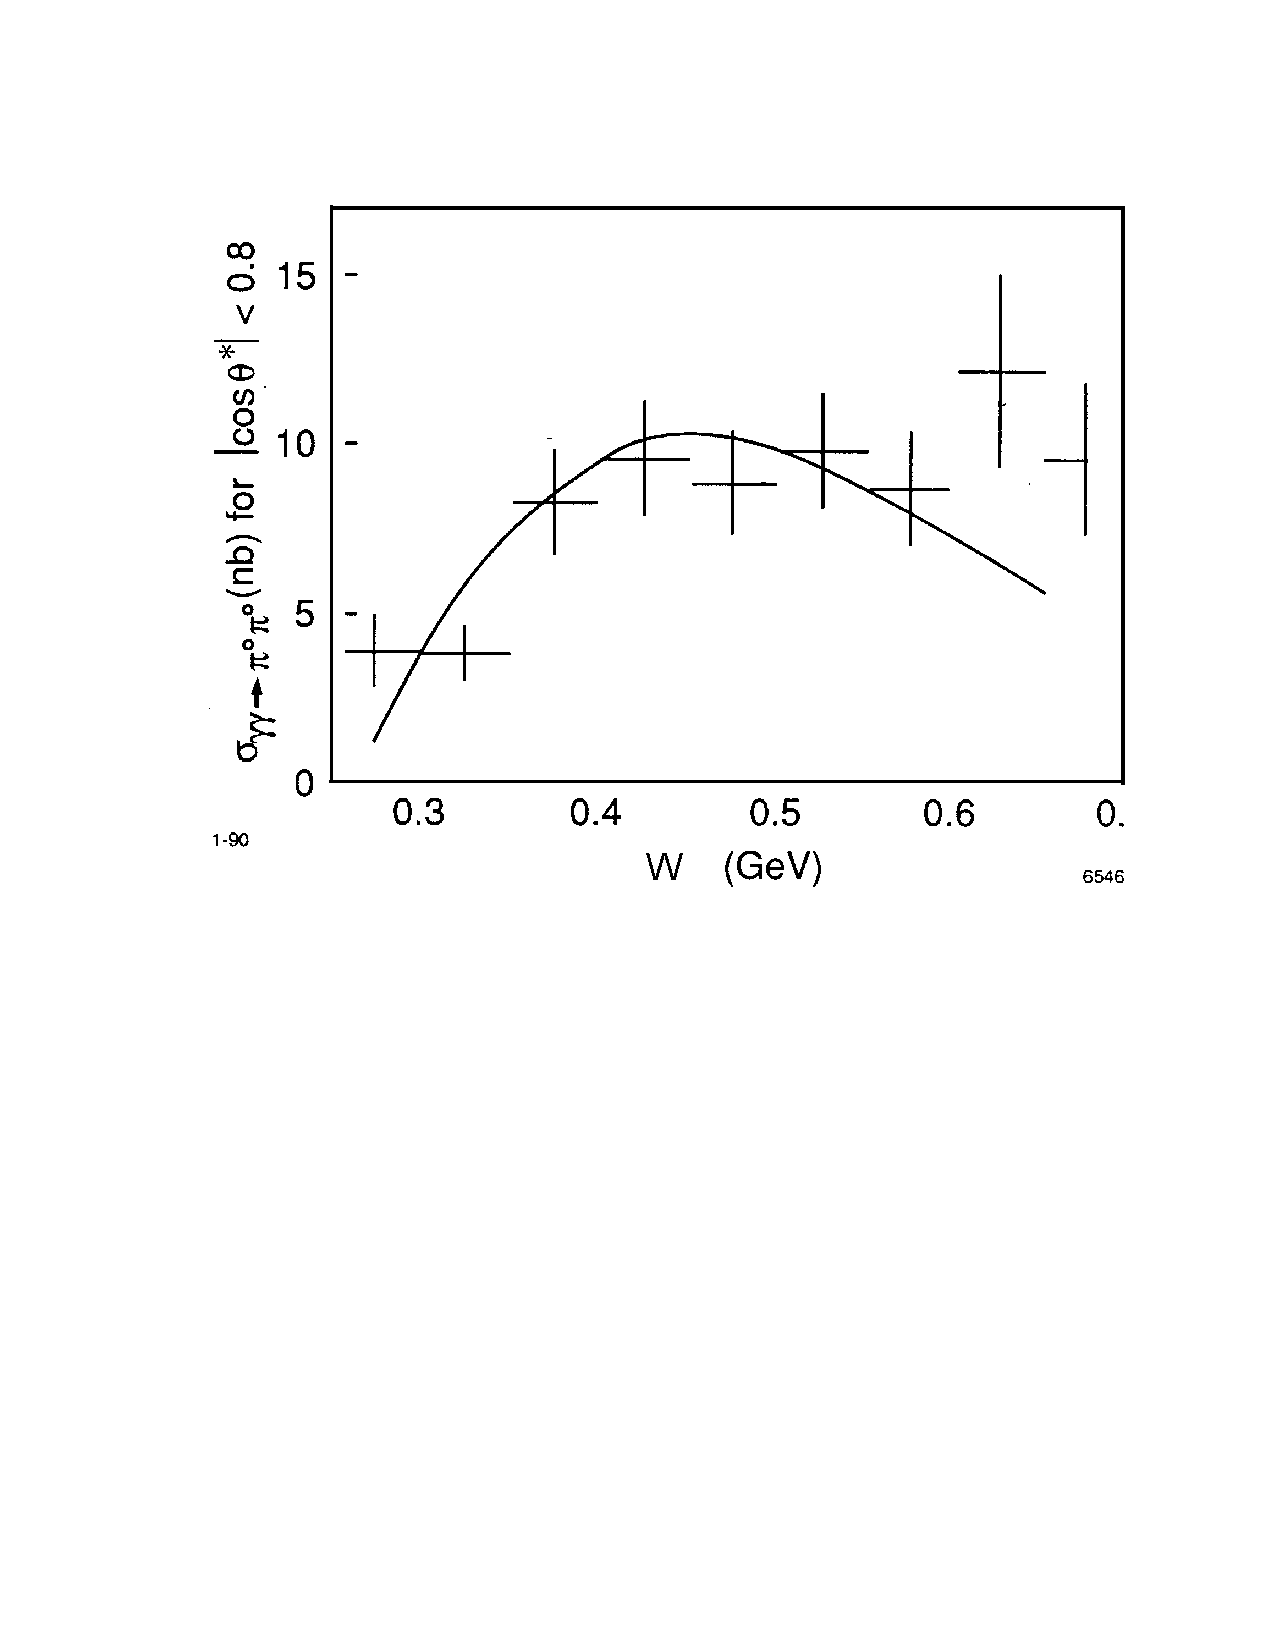
\includegraphics[height=5cm,angle=0]{figures/XBall.pdf}\\
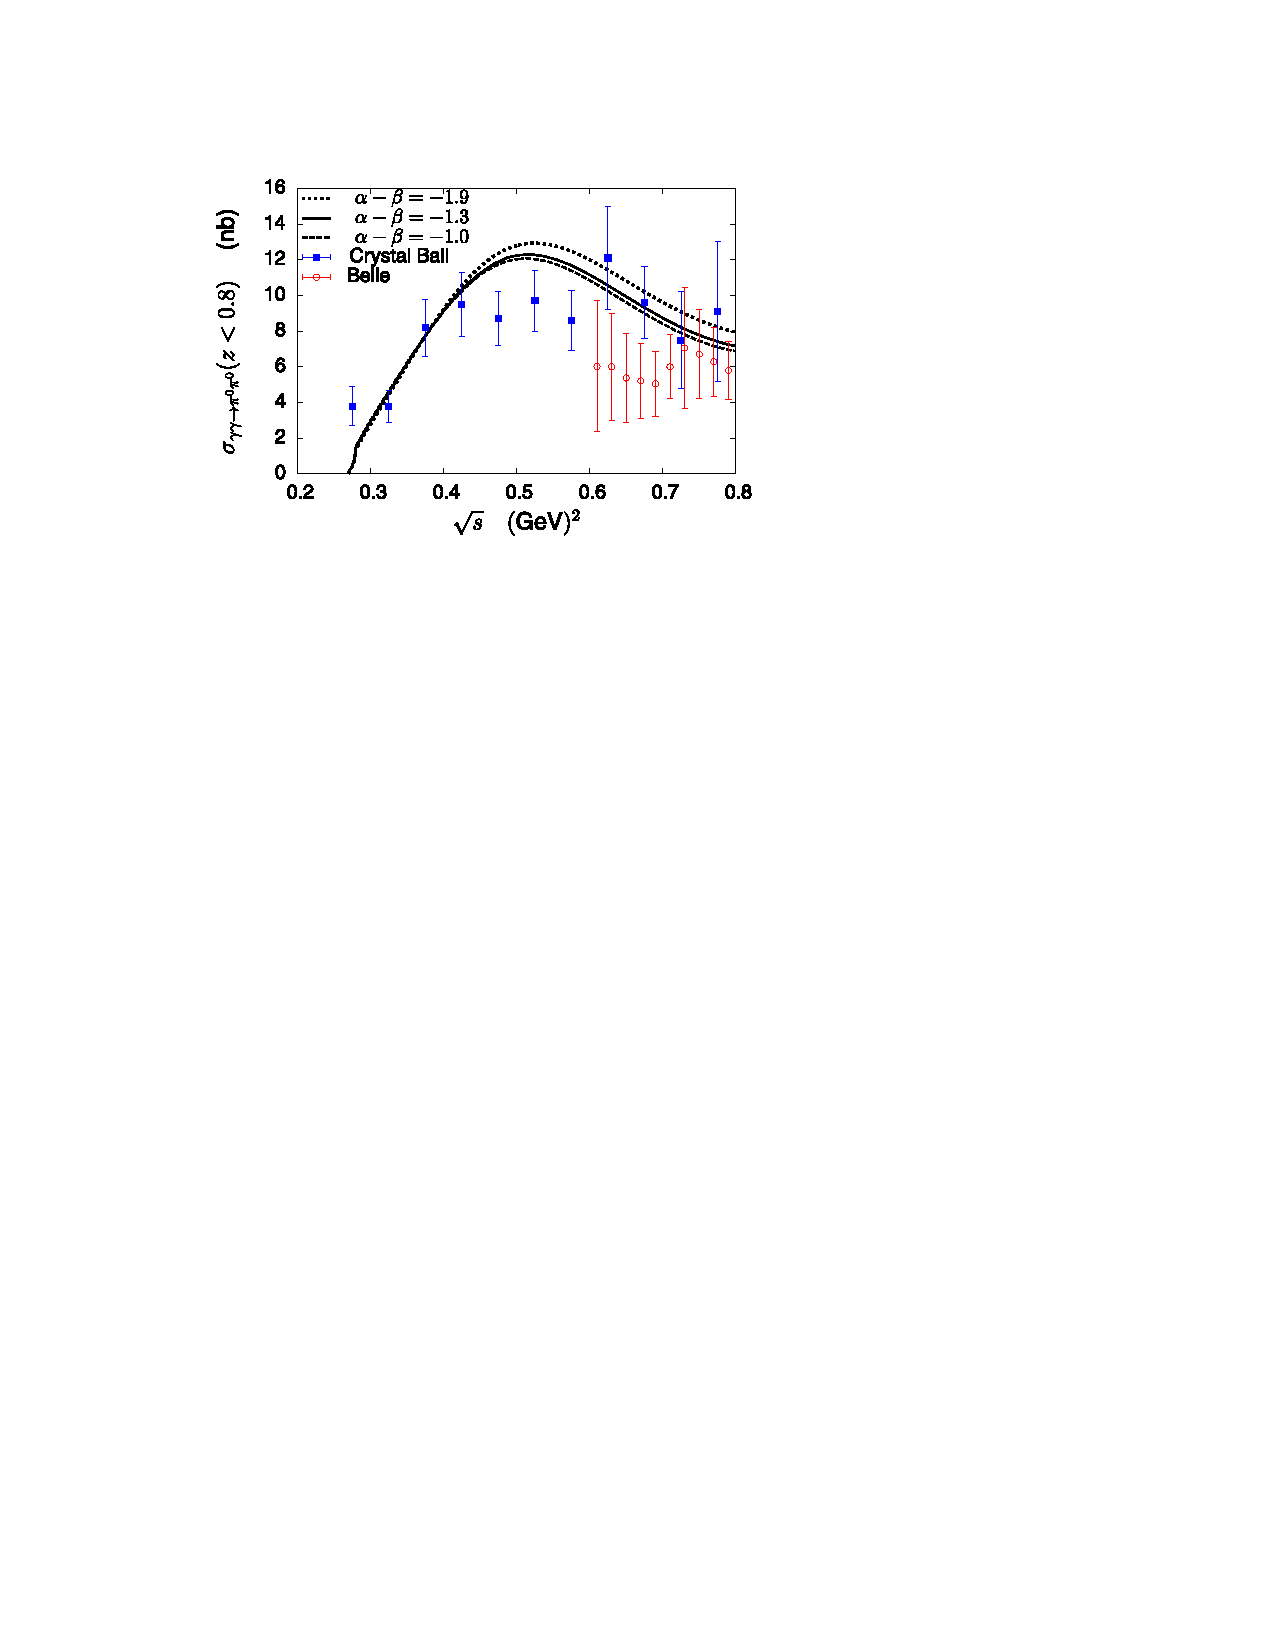
\includegraphics[height=6cm,angle=0]{figures/Fig-TP-5.pdf}\i
%\includegraphics[height=6cm,width=8cm,angle=0]{gA-Mpi-LHPC-band.pdf}
\end{center}
\caption{Left panel: experimental status; right panel: results from the 1990
XBall experiment. The lower panel shows the effect of $\pi^0$ polarizabilities
on the cross section ($\sqrt{s}=W_{\pi\pi}$) \cite{Moussallam:2013una} .
\label{fig:previousdata}}
\end{figure}

\section{Past Measurements}
Past measurements of the $\gamma\gamma\to \pi^0\pi^0$ cross section can be
summarized as follows:
\begin{enumerate}
    \item 
In the early 1990's measurements were made in $e^+e^-$ collisions at DESY
with the XBall detector at the DORIS-II storage ring, which are the only
available data for $W_{\pi\pi}<0.6{\rm~ GeV}$ \cite{Marsiske:1990hx}. 
\item In 2008-9, measurements were carried out by BELLE
for $0.6{\rm~ GeV}<W_{\pi\pi}<4.0 {\rm~ GeV}$ \cite{Mori:2007bu,Uehara:2008ep,Uehara:2009cka}. 
\end{enumerate}
As mentioned above, several works have made use of dispersion theory methods
(Oller and
Roca \cite{Oller:2008kf}, Dai and Pennington \cite{Dai:2016ytz}, and
in particular Moussallam \cite{Moussallam:2013una} who performed the
dispersive analysis where one of the photons has non vanishing
virtuality, which is particularly important for our case.) with those
available data. In particular these methods give results for the cross
section at small $W_{\pi\pi}$, but the poor accuracy of the data in
that region does not serve as a useful constraint that could improve
those analyses. On the other hand, the ChPT calculations carried out
at NNLO (Bellucci et al \cite{Bellucci:1994hx,Bellucci:1994eb} ) can
only be fitted to the low $W_{\pi\pi}$ data, and thus the uncertainty
in the determination of low energy constants is rather large. It is therefore
expected that accurate data at low $W_{\pi\pi}<0.6{\rm~ GeV}$ will
have a very big impact on both theoretical approaches, which together
may allow for an accurate description of the low energy Compton
amplitude, and for a first time experimental determination of the
polarizability.
